\documentclass[11pt,a4paper]{article}
\usepackage[margin=24mm]{geometry}
\usepackage{tikz}
\usetikzlibrary{positioning,arrows.meta}
\title{Seeded adversarial layouts: first verified experiment}
\author{HyMeKo research workspace}
\date{Created 2026-09-29 02:36 CEST}
\begin{document}
\maketitle
\paragraph{Scope and ETA.} A bounded research client generates grid layouts, compiles
them to the existing canonical IR, measures existing Graph searches, and exports
selected scenes through the existing Gazebo template pipeline. All simulation and
campaign execution occurs on Amaterasu. Estimated completion: 60--90 minutes, based
on implementation, focused tests, remote build, a 1000-candidate experiment and
artifact review. This is an estimate, not a deadline promise.
\paragraph{Ownership.} Core owns compilation, IDs, incidence indexing and semantic
hashes. Graph owns BFS, A* and their work counters. Emitter owns canonical HyMeKo
source output. Formats owns SDF generation. The example is experiment composition,
not a new production world model or graph engine. The simulator's dirty checkout
is not modified. The separate metaheuristics pilot has a different worker and files.
\paragraph{Files.} This plan's four files and:
\begin{itemize}
\item \texttt{hymeko\_formats/Cargo.toml}
\item \texttt{hymeko\_formats/examples/adversarial\_grid.rs}
\item \texttt{transforms/gazebo/queries.hymeko}
\item \texttt{transforms/gazebo/template.world.sdf}
\item \texttt{hymeko\_formats/tests/gazebo\_obstacles.rs}
\item \texttt{hymeko\_formats/tools/adversarial\_grid\_artifacts.py}
\item \texttt{hymeko\_formats/tools/run\_adversarial\_grid.sh}
\item \texttt{hymeko\_formats/tools/validate\_adversarial\_grid\_gazebo.py}
\item \texttt{hymeko\_emitter/src/emit\_hymeko.rs}: use the existing Core
\texttt{build\_path\_index} API; the pinned revision lacks the constructor currently called.
\item \texttt{hymeko\_query/tests/test\_prop\_witnesses.rs}: import the pinned
Core semantic digest under its existing versioned name so the integrated tests compile.
\item \texttt{reports/2026-09-29-adversarial-grid.md}
\end{itemize}
Generated artifacts live below that
report's companion directory. Cargo.lock changes only if dev-dependency bookkeeping
requires it. No CORE.YAML item is modified and no public Rust API changes.
\paragraph{Interfaces.} The example accepts output directory, seed count, candidates
per seed and bounded grid dimensions. Defaults: 16 by 16, 10 seeds, 100 proposals
per seed. Exported obstacle nodes inherit \texttt{gazebo\_static\_box} and carry
numeric x, y, z, size\_x, size\_y, size\_z attributes. The template adds static box
models with collision and visual geometry; scenes without such nodes retain their
existing semantics. Existing Graph and Emitter crates are reused as dev dependencies.
\paragraph{Method.} Keep start, goal, grid dimensions and wall count fixed. Use seeded
proposals; reject unreachable worlds. Baseline is the first feasible proposal;
the selected world maximizes existing Manhattan A* expanded-node count among the
same bounded proposal set. This is best-of-budget selection, not a universal
hardness proof. Existing BFS supplies a path witness; zero-heuristic search is a
secondary measurement. Save every proposal outcome, generation cost, configuration,
source and solver identity. Report selection cost separately from solving cost.
\paragraph{Validation.} Before the campaign: seed replay/variation, known-maze optimal
path, endpoint and obstacle validity, canonical source round trip and semantic hash,
SDF count/position/size checks. Run existing Gazebo template tests. Audit
\texttt{cargo tree -d}; Core/Graph identities must agree. On Amaterasu run the
campaign, validate SDF with installed Gazebo tooling, and run a finite headless
Gazebo simulation in its own transport partition. Check simulation time advanced,
expected obstacle count and poses, and no model-loading errors. Do not mistake
file parse success or process startup for a completed simulation.
\paragraph{Budget and risk.} Grid dimensions at most 16, at most 1000 proposals for
the first campaign, five-minute campaign cap, solver memory target below 2 GiB;
remote compilation uses at most two jobs and is logged separately. Gazebo uses a
finite iteration count and 60-second timeout. No paid model calls or GPU training.
Long paths must not hit the legacy u8 BFS distance cap. Source metadata must survive
round trip; EditorIR bridge metadata loss is why source-first compilation is used.
Disconnected proposals are rejected rather than scored as maximally hard. Tie
breaking and failure outcomes are recorded. Existing Amaterasu services are untouched.
\paragraph{Rollback and delivery.} Remove only task-added files and review the named
template/manifest diffs to revert them; preserve other workers' changes. No commit,
push or branch switching. Remote source copies are explicitly labeled build
snapshots of the local revision plus changes, not clean-clone release evidence.
Deliver JSON, plot, layout images and a path GIF; archive the report with the
existing report-sync tool. Record exact remote path, commands, logs and outcomes.
\begin{center}
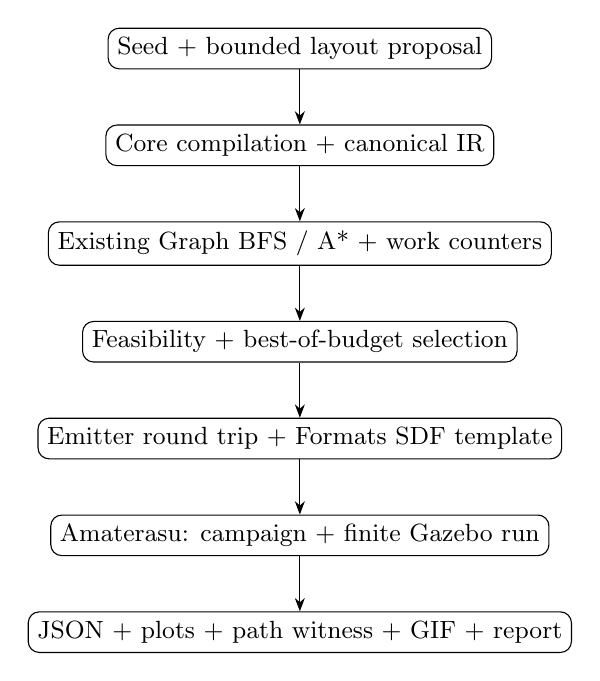
\begin{tikzpicture}[node distance=7mm, every node/.style={draw,rounded corners,align=center,font=\small}, >=Stealth]
\node (seed) {Seed + bounded layout proposal};
\node[below=of seed] (core) {Core compilation + canonical IR};
\node[below=of core] (graph) {Existing Graph BFS / A* + work counters};
\node[below=of graph] (select) {Feasibility + best-of-budget selection};
\node[below=of select] (emit) {Emitter round trip + Formats SDF template};
\node[below=of emit] (remote) {Amaterasu: campaign + finite Gazebo run};
\node[below=of remote] (results) {JSON + plots + path witness + GIF + report};
\draw[->] (seed)--(core);
\draw[->] (core)--(graph);
\draw[->] (graph)--(select);
\draw[->] (select)--(emit);
\draw[->] (emit)--(remote);
\draw[->] (remote)--(results);
\end{tikzpicture}

\end{center}
\end{document}
